\documentclass[a4paper]{article}

%% Language and font encodings
\usepackage[english]{babel}
\usepackage[utf8x]{inputenc}
\usepackage[T1]{fontenc}

%% Sets page size and margins
\usepackage[a4paper,top=3cm,bottom=2cm,left=3cm,right=3cm,marginparwidth=1.75cm]{geometry}

%% Useful packages
\usepackage{amsmath}
\usepackage{graphicx}
\usepackage[colorinlistoftodos]{todonotes}
\usepackage[colorlinks=true, allcolors=blue]{hyperref}

\title{Reporte de Evaluación 1}
\author{Valenzuela Terán Jonás}

\begin{document}
\maketitle
%-----------------------------------------------

\begin{center}

	
\includegraphics[height=4cm]{Unison.png}

\end{center}


\section{Introducción}

El propósito de la evaluación es verificar que conocemos y sabemos manejar las herramientas que hemos aprendido a utilizar en clase. En este caso, se utilizan para hacer un análisis de datos acerca de el nivel del mar, salinidad y temperatura del agua para encontrar la relación que guardan. Esto es posible haciendo uso de representaciones gráficas que ayudan a interpretar los datos,

\begin{center}

	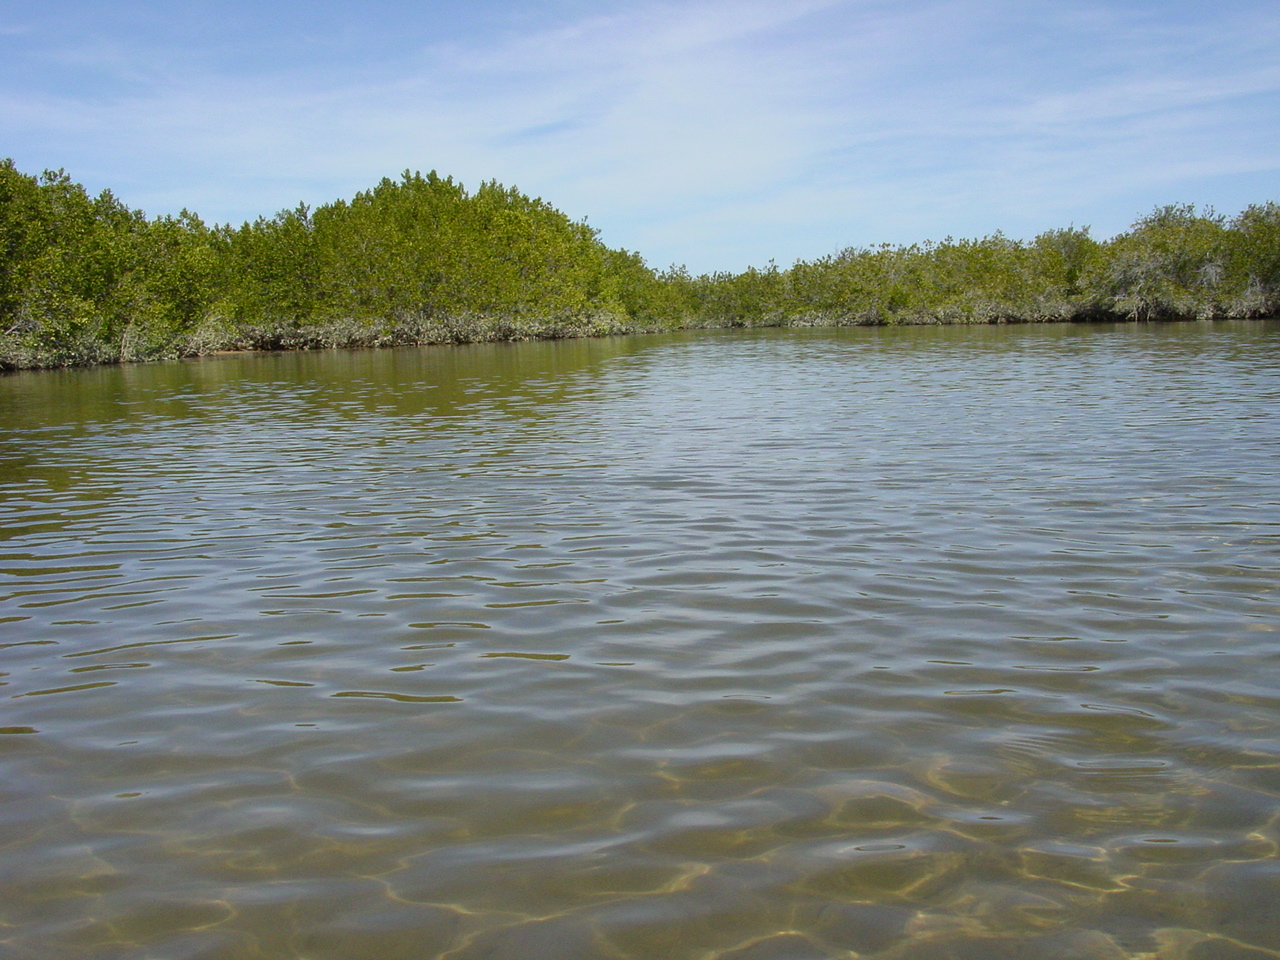
\includegraphics[height=5cm]{manglar.jpg}
    
    \textit{Manglar El Sargento  -Carlos Lizarraga Celaya}
    
\end{center}


\section{Recuperación y limpieza de datos}

Los datos fueron tomados en el manglar El Sargento y proporcionados por el profesor, se utilizaron comandos de \textit{emacs} para adaptar el formato, en si, los datos necesitaron solo de cambios menores, de la separación entre variables, con comas y espacios.

\section{Análisis de datos}

Una vez que los datos se encuentran en el formato deseable,  cada archivo de datos es asignado a un dataframe en \textit{python}, con entorno de programación \textit{jupyter notebook}, donde se importan bibliotecas útiles como numpy \textit{}para herramientas numéricas, \textit{pandas} para estadística, \textit{datetime} para formato de tiempo, \textit{matplotlib} y \textit{seaborn }para gráficas.

Se asignó un dataframe que contiene la información de interés para esta práctica, que es la fecha, nivel del mar, salinidad y temperatura, después se representó con boxplots de cada variable, regresiones lineales de Pearson y gráficas de variable contra tiempo individuales y superpuestas.

Para la lectura de datos, se ignoraron las mediciones que no coincidieran en el tiempo de un archivo a otro, y los encabezados, para asignarlos manualmente: (>> indica una instrucción o línea)

\begin{verbatim}


>> df1 = pd.read_csv('sargento_201117.csv', names=['Date-Time', 'AbsPres', 'Temp', 'WaterLevel'], skiprows=2, 
skipfooter=1, sep=',', engine='python')
>> df2 = pd.read_csv('sargento-salinidad-201117.csv', names=['Date-Time', 'Cond-High-Rng', 
'Temp', 'SpecificC', 'Salinity'], skiprows=2, sep=',')
>> df2 = df2.drop(df2.index[:1])
\end{verbatim}

Después, se creó un nuevo dataframe con la información de interés:

\begin{verbatim}
>> df3 = pd.concat([df1['Date-Time'], df1['WaterLevel'],  df2['Salinity'], df1['Temp']], axis=1, keys=['Date-Time', 'WaterLevel', 'Salinity','Temp'])
\end{verbatim}

Se creó la variable temporal \textit{Ndate} y \textit{month} para poder trabajar por mes en los boxplots:

\begin{verbatim}
>> df3['Ndate'] = pd.to_datetime(df3['Date-Time'], format='%m/%d/%Y/%H:%M:%S')
>> df3['month'] = df3['Ndate'].dt.month
\end{verbatim}

Continuamente se utilizaron las funciones \textit{head()} y \textit{tail()} para comprobar el formato de los datos. Una vez comprobados, se crearon los boxplot de la siguiente manera:

\begin{verbatim}
>> import seaborn as sns

>> ax = sns.boxplot(x="month", y="WaterLevel", data=df3)
>> plt.show()
\end{verbatim}

La regresión lineal de Pearson, en general, fue creada con el código:

\begin{verbatim}
>> sns.set(style="darkgrid", color_codes=True)

>> g = sns.jointplot("WaterLevel", "Salinity", data=df3, kind="reg",
                   color="r", size=7)
>> plt.show(g)
\end{verbatim}

Se crearon gráficas de la variable con respecto al tiempo, creando nuevos dataframe, con:

\begin{verbatim}
>> df4 = df3[['Date-Time','WaterLevel']]
>> plt.figure(); df4.plot(x='Date-Time'); plt.legend(loc='best')
>> plt.title('Variación del Nivel del mar')
>> plt.ylabel('Metros')
>> plt.xlabel('Tiempo')
>> plt.grid(True)
>> plt.show()
\end{verbatim}

Después se realizó una superposición de las variables contra el tiempo:

\begin{verbatim}
>> df7 = df3[['Date-Time','WaterLevel','Salinity']]
>> plt.figure(); df7.plot(x='Date-Time'); plt.legend(loc='best')
>> plt.title('Variación del Nivel del mar y Salinidad')
>> plt.xlabel('Tiempo')
>> plt.grid(True)
>> plt.show()
\end{verbatim}

Y finalmente, se utilizó la función xlim para delimitar un rango de tiempo más corto:

\begin{verbatim}
>> df9 = df3[['Date-Time','WaterLevel','Salinity']]
>> df9n= df9.iloc[1:525]
>> plt.figure(); df9n.plot(x='Date-Time'); plt.legend(loc='best')
>> plt.title('Variación del Nivel del mar y Salinidad a 5 días')
>> plt.xlabel('Tiempo')
>> plt.grid(True)
>> plt.show()
\end{verbatim}



\section{Resultados}

A continuación se muestran las representaciones gráficas obtenidas:

\begin{center}
	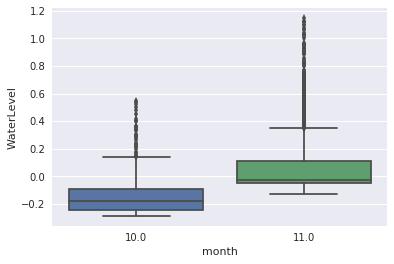
\includegraphics[height=4cm]{Boxplot1.png}
    
    \textit{Boxplot de Nivel del Mar por mes}
\end{center}

\begin{center}
	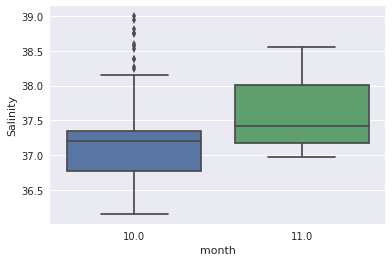
\includegraphics[height=4cm]{Boxplot2.png}
    
    \textit{Boxplot de Salinidad por mes}
\end{center}

\begin{center}
	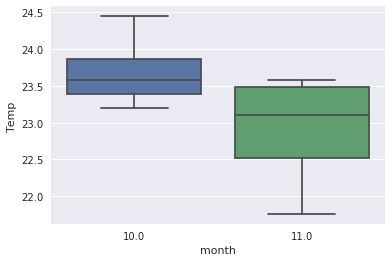
\includegraphics[height=4cm]{Boxplot3.png}
    
    \textit{Boxplot de Temperatura por mes}
\end{center}

Se observa a través de los boxplots, que al comparar noviembre con octubre en general, el nivel del agua y salinidad se eleva, mientras que las temperaturas disminuyen.

\begin{center}
	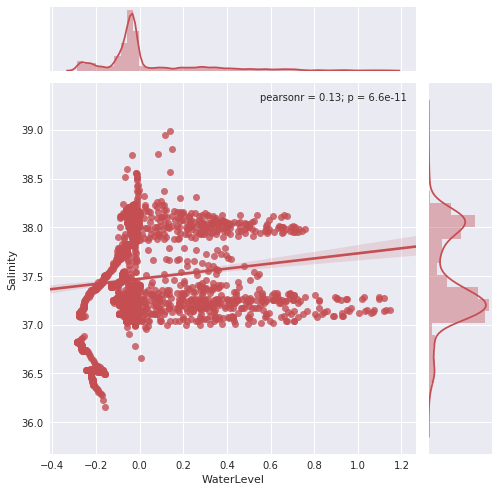
\includegraphics[height=5cm]{Regresion1.png}
    
    \textit{Regresión lineal de Salinidad contra Nivel del mar}
\end{center}

\begin{center}
	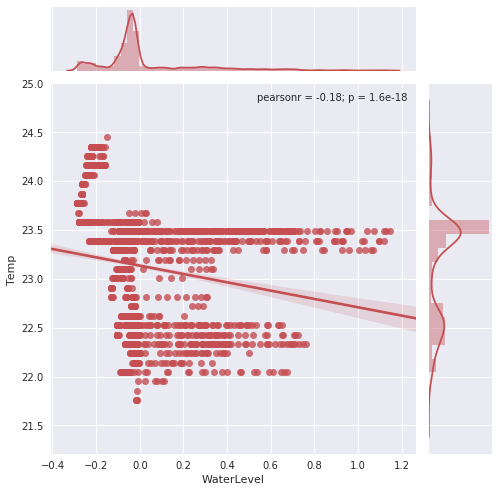
\includegraphics[height=5cm]{Regresion2.png}
    
    \textit{Regresión lineal de la Temperatura contra Nivel del mar}
\end{center}

\begin{center}
	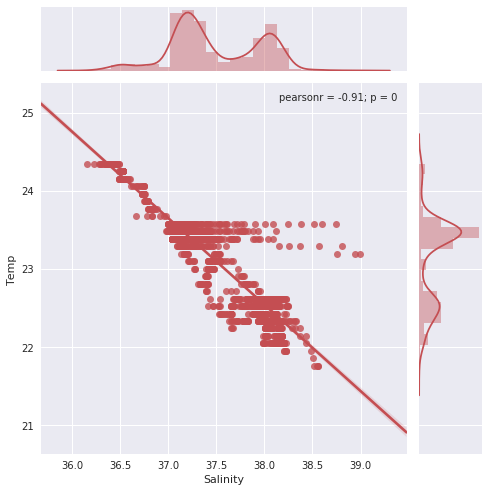
\includegraphics[height=5cm]{Regresion3.png}
    
    \textit{Regresión lineal de Temperatura contra Salinidad}
\end{center}

Se puede notar a través de esta representación que el único par de variables que se cuentan con una relación aproximadamente real es la Salinidad y Temperatura.

\begin{center}
	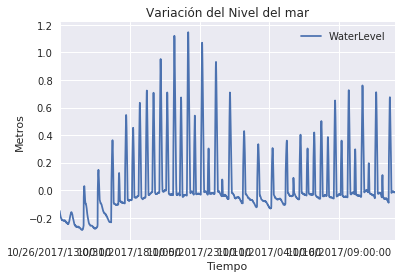
\includegraphics[height=4cm]{Gr1.png}
    
    \textit{Gráfica de Nivel del mar contra tiempo}
\end{center}

\begin{center}
	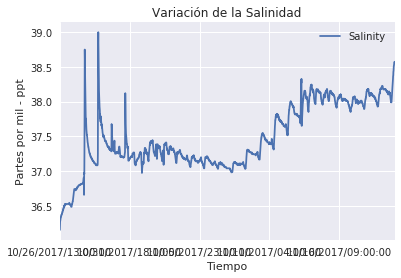
\includegraphics[height=4cm]{Gr2.png}
    
    \textit{Gráfica de Salinidad contra tiempo}
\end{center}

\begin{center}
	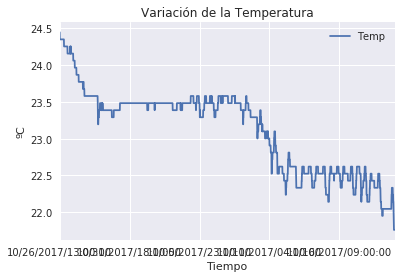
\includegraphics[height=4cm]{Gr3.png}
    
    \textit{Gráfica de Temperatura contra tiempo}
\end{center}

Se muestra mucha variación de cada variable con respecto al tiempo, para poder encontrar una relación, resulta más conveniente hacer una superposición.

\begin{center}
	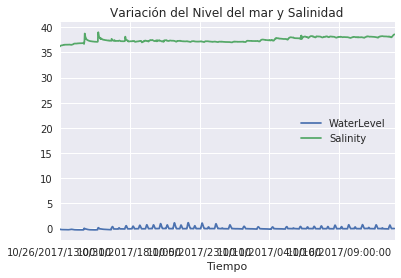
\includegraphics[height=4cm]{Gr4.png}
    
    \textit{Gráfica del Nivel del mar y Salinidad contra tiempo}
\end{center}

\begin{center}
	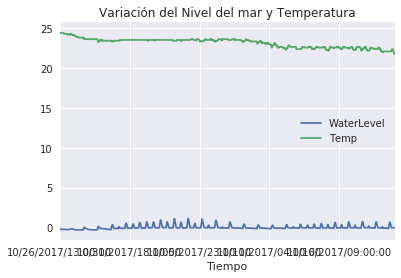
\includegraphics[height=4cm]{Gr5.png}
    
    \textit{Gráfica de Nivel del mar y Temperatura contra tiempo}
\end{center}

Aun no es claro si existe relación o no a través de este tipo de gráfica, debemos analizar un intervalo más pequeño de tiempo.

\begin{center}
	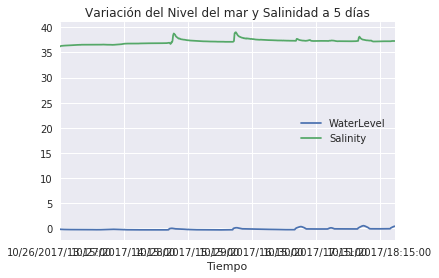
\includegraphics[height=4cm]{Gr6.png}
    
    \textit{Gráfica del Nivel del mar y Salinidad contra tiempo en 5 días}
\end{center}

\begin{center}
	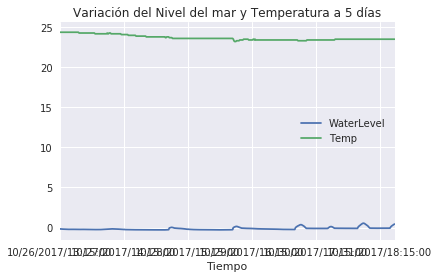
\includegraphics[height=4cm]{Gr7.png}
    
    \textit{Gráfica de Nivel del mar y Temperatura contra tiempo en 5 días}
\end{center}

Ahora es notable la relación entre el Nivel del mar y la Salinidad, cuando una variable aumenta, la otra también, pero con magnitud diferente.

\section{Final}

Ya terminada la actividad, se guardaron todos los archivos en un solo directorio (Evaluación1), y se guardaron en la plataforma de github, siendo útil para futura consulta, y revisar los métodos aprendidos para lectura, acomodo y graficación de datos.
\end{document}